\documentclass{beamer}

\usepackage[utf8]{inputenc}
\DeclareUnicodeCharacter{2212}{-}
\usecolortheme{beaver}
\usepackage{caption}
\usepackage{tabularx}
\usepackage{amsmath}
\usepackage{amsfonts}
\usepackage{amssymb}
\usepackage{subcaption}
\usepackage{mathtools}
\usepackage{graphicx}
\usepackage{todonotes}
\usepackage[style=verbose, backend=biber]{biblatex}

\DeclarePairedDelimiter\norm{\lVert}{\rVert}%

\addbibresource{references.bib}

\setbeamertemplate{navigation symbols}{}

\begin{document}

\title{Simulation methods for Causal Effect Estimation}
\date{}
\maketitle

\begin{frame}
	\frametitle{Index}
	\begin{itemize}
		\item Potential Outcome Framework
		\item Problem Statement
		\item Monte Carlo based
			\begin{itemize}
				\item Placebo Design
				\item Structured Design
				\item Bootstrapping
			\end{itemize}
		\item Generative Deep Learning based
			\begin{itemize}
				\item Wasserstein Generative Adversarial Networks (GANs)
				\item Variational Autoencoders (VAEs)
			\end{itemize}
	\end{itemize}
\end{frame}

\begin{frame}
	\frametitle{Potential Outcomes Framework}
	Average Treatment Effect (ATE): $ \mathbb{E}[Y_t(u) - Y_c(u)] $ \newline
	Conditional ATE: $ \mathbb{E}[Y_t(u) - Y_c(u) | u=u_i ] $

	\begin{columns}
		\begin{column}{0.5 \textwidth}
		\begin{table}
			\centering
			\begin{tabularx}{\linewidth}{| c | c | c | c |} 
			\hline 
			& $ Y_{t}(u) $  & $ Y_{c}(u) $ & \\
			\hline
				Joe    & 130     & 135    & −5 \\
				Mary   & 140     & 150    & −10 \\
				Sally  & 135     & 125    & 10 \\
				Bob    & 135     & 150    & −15 \\
			\hline
			\hline
			\end{tabularx}
		\end{table}
		\end{column}
		\begin{column}{0.5 \textwidth}
		\begin{table}
			\centering
			\begin{tabularx}{\textwidth}{| c | c | c | c |} 
			\hline 
			& $ Y_{t}(u) $  & $ Y_{c}(u) $ & \\
			\hline
				Joe    & 130     & ? & ? \\
				Mary   & ? & 150    &  ? \\
				Sally  & ? & 125    &  ? \\
				Bob    & 135     & ? & ? \\
			\hline
			\hline
			\end{tabularx}
		\end{table}
		\end{column}
	\end{columns}	
	\footnotetext[1]{https://en.wikipedia.org/wiki/Rubin\_causal\_model}
\end{frame}


\begin{frame}
	\frametitle{Problem Statement}
	\begin{itemize}
		\item Lots of different estimators for treatment effect eg. Propensity score matching, Double ML, BART, Causal Forests. \todo[inline]{Check how do these methods work}
		\item Estimators have similar asymptotic properties but difference finite-sample properties.
	\end{itemize}
	\begin{table}[h!]
		\centering
		\begin{tabularx}{\textwidth}{||c c c||} 
		 \hline
		 \textbf{Estimators}  & \textbf{ATE Estimate} & \textbf{Std. Dev.} \\
		 \hline\hline
		 Difference of Means & 886.30 & 277.37 \\ 
		 Double Machine Learning & 370.94 & 394.68 \\
		 Causal Bart & 818.79 & 184.46 \\
		 Propensity Score Matching & 1079.13 & 158.59 \\
		 \hline
		\end{tabularx}
		\caption*{ATE estimates on the National Support Work Demonstration temporary employment program and income dataset \footcite{parikh2022evaluating}}
		\label{table:estimates}
	\end{table}
\end{frame}

\begin{frame}
	\frametitle{Problem Statement}
	\begin{itemize}
		\item In correlational models, performance of an estimator can be measured by
			splitting data into training and test sets.
		\item True causal effect is unknown for most datasets, so estimator performances
			can't be compared for a given dataset.
		\item Solution: Simulate data with same statistical properties as the original dataset, and compare performance of the estimators.
		\item Requires assumptions to be made. \todo[inline]{Add examples of kinds of assumptions required}
	\end{itemize}
\end{frame}

\begin{frame}
	\frametitle{Finite sample performance comparison using RCTs}
	\begin{itemize}
		\item Uses data from Randomized Control Trials(RCT) for true causal effect.
		\item Observational sampling from RCT data to create simulated
			observational datasets.
		\item Estimation is done on the simulated data and compared to the true effect.
	\end{itemize}

	\begin{figure}
		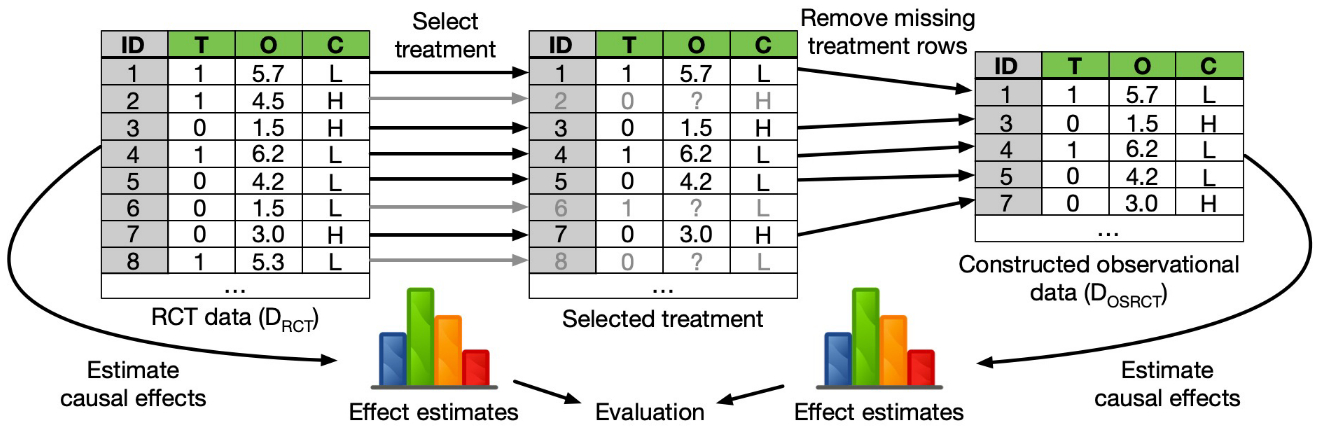
\includegraphics[width=\textwidth]{fig_osrct.jpg}
	\end{figure}
	\footnotetext{Gentzel, Amanda M., Purva Pruthi, and David Jensen. "How and why to use experimental data to evaluate methods for observational causal inference." International Conference on Machine Learning. PMLR, 2021.}
\end{frame}

\begin{frame}
	\frametitle{Finite sample performance comparison using RCTs}
	\begin{itemize}
		\item Use some of the covariates (which also affect the outcome) to bias the random
			selection.
		\item Using the baised treatment selection, sample from the RCT dataset.
		\item Gives a biased observational dataset, where the bias covariates are the 
			confounders.
		\item All the estimators perform reasonably well on all the datasets.
	\end{itemize}

	\begin{figure}
		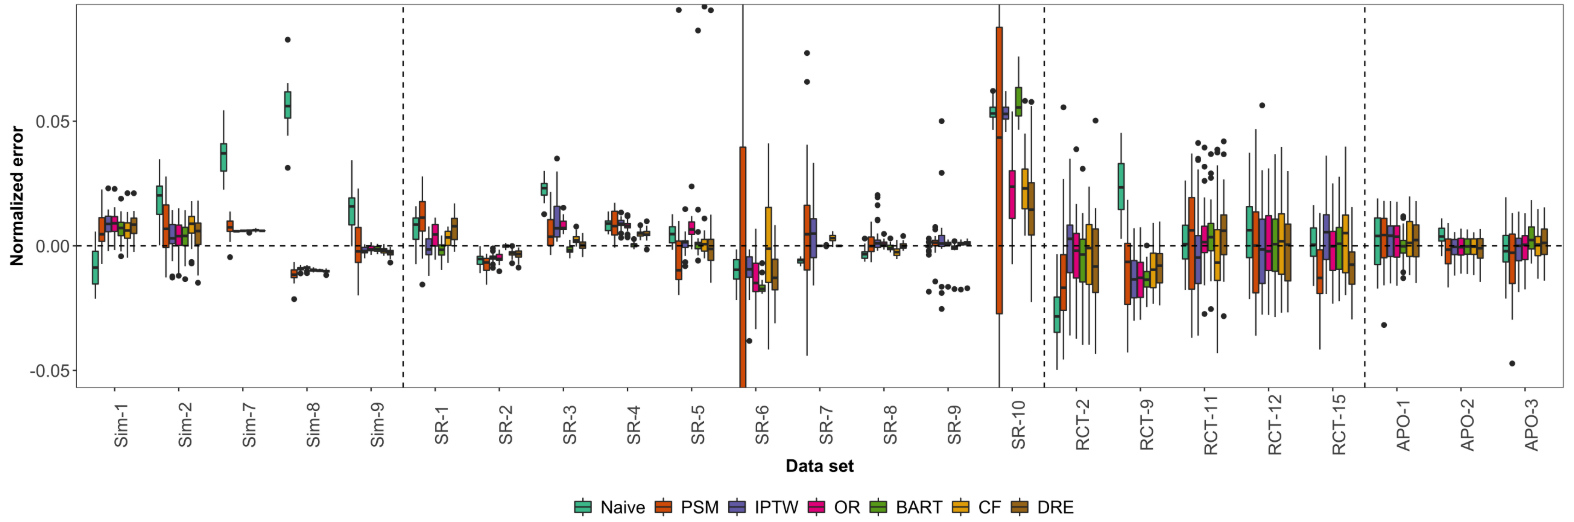
\includegraphics[width=\textwidth]{fig_rct.jpg}
	\end{figure}

\end{frame}

\begin{frame}
	\frametitle{Placebo Design}
	\begin{itemize}
		\item Only useful when the dataset arms are placebo vs treatment.
		\item Use the placebo arm as the ground truth with known treatment effect = $ 0 $.
		\item Use the estimators to estimate the effect in the placebo arm and compare results.
	\end{itemize}
	\footnotetext{Huber, Martin, Michael Lechner, and Conny Wunsch. "The performance of estimators based on the propensity score." Journal of Econometrics 175.1 (2013): 1-21.}
\end{frame}

\begin{frame}
	\frametitle{Structured Design}
	\begin{itemize}
		\item Assume a data generating structure i.e. DAG.
		\item Use the DAG to compute the true causal effect under structure assumptions.
		\item Compare estimators to the effect estimated from DAG.
	\end{itemize}
	\footnotetext{Busso, Matias, John DiNardo, and Justin McCrary. "New evidence on the finite sample properties of propensity score reweighting and matching estimators." Review of Economics and Statistics 96.5 (2014): 885-897.}
\end{frame}

\begin{frame}
	\frametitle{Mostly Harmless Simulations}
	\begin{itemize}
		\item Both the methods don't really work, the estimator performances are very
			dependent on the assumptions that we make.
		\item Bootstrapping might just be a better option.
		\item Unrealistic assumptions on the data generating process lead to unreliable results.
	\end{itemize}
	\footnotetext{Advani, Arun, Toru Kitagawa, and Tymon Słoczyński. "Mostly harmless simulations? Using Monte Carlo studies for estimator selection." Journal of Applied Econometrics 34.6 (2019): 893-910.}
\end{frame}

\begin{frame}
	\frametitle{Using Wasserstein GANs}
	\begin{itemize}
		\item Not a single estimator which works well for all.
		\item Systematic simulation studies can be helpful for selecting methods.
		\item Generated data closely resembles the actual data.
		\item DGP like kernel desnity doesn't work because of oversmooth in case of finite samples. Bootstrp doesn't replace the original samples and there is overlap.
	\end{itemize}
	\footnotetext{Athey, Susan, et al. "Using wasserstein generative adversarial networks for the design of monte carlo simulations." Journal of Econometrics (2021)}
\end{frame}

\begin{frame}
	\frametitle{Using VAEs}
	\begin{itemize}
		\item Relaxes conditional ignorability. Allows users to specify treatment effects and confounding bias.
		\item Paper only considers the problem of estimating ATE i.e $ \tau = \mathbb{E}[Y(1) - Y(0)] $.
		\item Method to generate synthetic data with two features: 1) User-specified causal treatment effect, heterogeneity, and endogeneity. 2) simulated samples that are stochastically indistinguishable from the observed data sample of interest.
	\end{itemize}
	\footnotetext{Parikh, Harsh, et al. "Evaluating Causal Inference Methods." arXiv preprint arXiv:2202.04208 (2022)}
\end{frame}

\begin{frame}
	Assumed data generating process:
	\begin{equation}
		\begin{split}
			\{ \epsilon_{X, i}, \epsilon_{Z, i}, \epsilon_{Y, i} \}_{i=1}^N & \sim \mathcal{N}(\mathbf{0}, \mathbf{1}) \\
			\{ U_i \} & \sim \mathcal{N}(0, 1) \\
			X_i & \sim \phi_X(\epsilon_(X, i) \\
			Z_i & \sim \phi_Z(X_i, U_i, \epsilon_{Z, i}) \\
			Y_i(1) & \sim \phi_{Y_i(1)} (X_i, U_i, \epsilon_{Y, i}) \\
			Y_i(0) & \sim \phi_{Y_i(0)} (X_i, U_i, \epsilon_{Y, i})
		\end{split}
	\end{equation}
	User defined inputs/assumptions:
	\begin{equation}
		\begin{split}
			f(x) &= \mathbb{E}[Y(1) - Y(0) | X=x] \\
			g(x, z) &= \mathbb{E}[Y(z) | X=x, Z=z] - \mathbb{E}[Y(z) | X=x, Z=1-z] \\
		\end{split}
	\end{equation}
\end{frame}
\begin{frame}
	\begin{equation}
		\begin{split}
			\mathbf{\min}_{\theta} & \mathbb{E}[d((X, Y, Z), (X', Y', Z'))] + \alpha \norm{\mathbb{E}[Y'(1) - Y'(0) | X' = x'] -f(x') } \\
						& + \beta \norm{\mathbb{E}[Y'(z') | X'=x', Z'=z] - \mathbb{E}[Y'(z') | X'=x', Z'=1-z'] -g(x', z')}
		\end{split}
	\end{equation}

	\begin{itemize}
		\item First term: Some distance measure on the distributions.
		\item Second term: Difference between the user-specified causal effect and expected from the generated data.
		\item Third term: Difference between estimated confounding and user-specified.
	\end{itemize}
	Two VAEs, first one to learn $ P(X | Z) $ and second one to learn $ P((Y(1), Y(0)) | X, Z) $.
\end{frame}
\begin{frame}
	\begin{figure}
		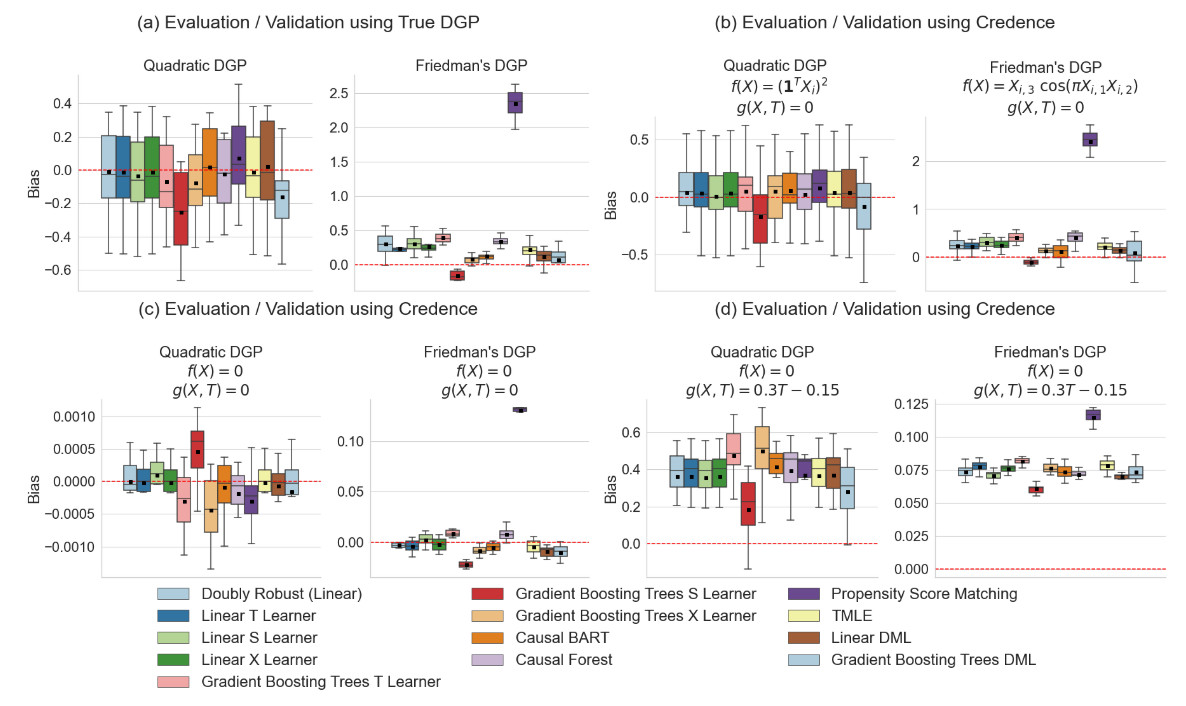
\includegraphics[width=\textwidth]{fig_3.jpg}
	\end{figure}
\end{frame}
\begin{frame}
	\begin{figure}
		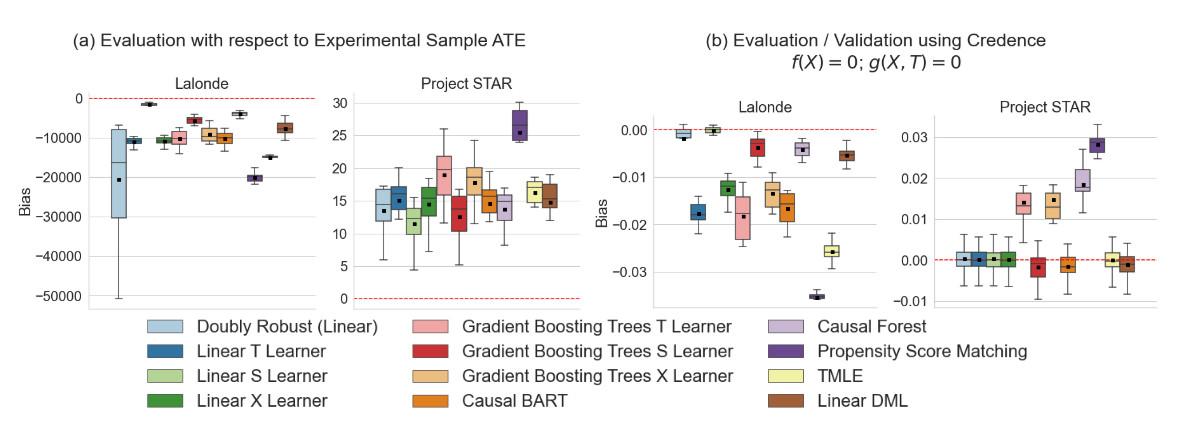
\includegraphics[width=\textwidth]{fig_4.jpg}
	\end{figure}
\end{frame}

\begin{frame}
	\frametitle{Conclusion}
	\begin{itemize}
		\item Simulations can be used to compare performance for selecting estimator.
		\item No assumption free method, different assumptions needed for different methods.
	\end{itemize}
\end{frame}

\end{document}
